\documentclass{beamer}
\usepackage[utf8]{inputenc}
\usepackage[italian]{babel}
\usepackage{amsmath}
\usepackage{amsfonts}
\usepackage{amssymb}
\usepackage{graphicx}
\usepackage[linesnumbered]{algorithm2e}
\usepackage{float}
\usepackage{mathtools}
\usepackage{subcaption}
\usepackage{wrapfig}
\usepackage{fancyhdr}
\usepackage{xcolor}
\usepackage{hyperref}
\usepackage{listings}
\usepackage{adjustbox}
\usepackage{enumerate}
\usepackage{booktabs}

\newcommand{\figcen}[2]{
 \begin{figure}
  \begin{center}
   \includegraphics[width=#1]{#2}
  \end{center}
 \end{figure}
}
\newtheorem{proposition}[theorem]{Proposizione}
\newtheorem{teorema}[theorem]{Teorema}

\definecolor{codeblue}{rgb}{0.21, 0.46, 0.80}
\definecolor{backcolour}{rgb}{0.95,0.95,0.92}
\definecolor{monokai@black}{HTML}{2C2C2A}
\definecolor{monokai@gray}{HTML}{524F52}
\definecolor{monokai@magenta}{HTML}{D33682}
\definecolor{monokai@blue}{HTML}{004C99}

\lstdefinestyle{sql}{
	frame=tb,
	language=SQL,
	backgroundcolor=\color{backcolour},
	aboveskip=3mm,
	belowskip=3mm,
	showstringspaces=false,
	basicstyle={\small\ttfamily},
	breaklines=true,
	breakatwhitespace=true,
	tabsize=1,
	keywordstyle=\color{codeblue},
	stringstyle=\color{monokai@magenta}\ttfamily,
	identifierstyle=\color{monokai@black},
	commentstyle=\color{monokai@blue},
	emphstyle=\color{monokai@red},
	columns=fullflexible
}
\lstdefinestyle{R}{
	frame=tb,
	language=R,
	backgroundcolor=\color{backcolour},
	aboveskip=3mm,
	belowskip=3mm,
	showstringspaces=false,
	basicstyle={\small\ttfamily},
	breaklines=true,
	breakatwhitespace=true,
	tabsize=1,
	keywordstyle=\color{codeblue},
	stringstyle=\color{monokai@magenta}\ttfamily,
	identifierstyle=\color{monokai@black},
	commentstyle=\color{monokai@blue},
	emphstyle=\color{monokai@red},
	columns=fullflexible
}

\usetheme[block = fill, progressbar=foot]{metropolis}
\setbeamertemplate{navigation symbols}{}
\setbeamertemplate{blocks}[rounded]


\title{Clustering studenti informatica}
\date{\today}
\author{Tommaso Ceccarini, Filippo Mameli}
    
\begin{document}
        
    \maketitle

    \section{Introduzione}
    
    \begin{frame}{Il dataset}

        Il dataset che abbiamo analizzato contiene dati sulle carriere accademiche degli studenti del corso di laurea di informatica dell'università degli studi di Firenze e il loro voto conseguito 
        al test di ingresso.
        \begin{itemize}
            \item Coorte: Anno di immatricolazione
            \item Crediti totali: Numero crediti complessivi dello studente
            \item Crediti con voto: Numero di crediti assegnati allo studente per esami con votazione in trentesimi (tutti tranne Inglese)
            \item Voto medio: Media pesata dei voti degli esami sostenuti
        \end{itemize}
    \end{frame}

    \begin{frame}{Il dataset}
        \begin{itemize}
            \item Valutazione conseguita all'esame
            \item Data in cui lo studente ha sostenuto l'esame
        \end{itemize}
        Gli esami sono Algoritmi e strutture dati (ASD), Programmazione (PRG), Architetture degli elaboratori (ARC), Analisi I (ANI), Matematica discreta e logica (MDL) e Inglese.
        \begin{itemize}
            \item Punteggio conseguito al test di ingresso.
        \end{itemize}
    \end{frame}

    \section{Gestione dei dati}

    \begin{frame}{La gestione dei dati}
        Le principali operazioni effettuate sul dataset sono:
        \begin{itemize}
            \item eliminare gli studenti che hanno sostenuto solo inglese
            \item riportare tutti gli attributi relativi alle date degli esami nel formato YYYY-MM-DD
        \end{itemize}
    \end{frame}

\begin{frame}[fragile]{Creazione table}
\begin{lstlisting}[style=sql]
CREATE TABLE 'studenti' (
  'coorte' int(11),
  'crediti_totali' int(11),
  'crediti_con_voto' int(11),
  'voto_medio' int(11),
  'ASD' int(11),
  'data_ASD' text,
    ...
  'data_INGLESE' text,
  'TEST' int(11)
) ENGINE=InnoDB

LOAD DATA INFILE 'studenti.csv' INTO TABLE studenti
  FIELDS TERMINATED BY ',' ENCLOSED BY '"'
  LINES TERMINATED BY '\r\n'
  IGNORE 1 LINES; 
\end{lstlisting}
\end{frame}

\begin{frame}[fragile]{Update tabella}
\begin{lstlisting}[style=sql]
update dmo.studenti set data_ARC = '0000-00-00' where data_ARC='0'; 
update dmo.studenti set data_ASD = '0000-00-00' where data_ASD='0'; 
update dmo.studenti set data_PRG = '0000-00-00' where data_PRG='0'; 
update dmo.studenti set data_ANI = '0000-00-00' where data_ANI='0'; 
update dmo.studenti set data_MDL = '0000-00-00' where data_MDL='0';
update dmo.studenti set data_INGLESE = '0000-00-00' where data_INGLESE = '0';
\end{lstlisting}
\end{frame}

\section{Analisi dei dati}

\begin{frame}{Analisi dei dati}
    Tabella di correlazione
    \begin{table}[H]
        \centering
        \resizebox{\textwidth}{!}{
        \begin{tabular}{@{}llllllllllll@{}}
                           & coorte   & crediti totali & crediti con voto  & voto medio  & ASD      & ARC      & PRG     & ANI     & MDL      & ING & TEST    \\ \midrule
        coorte             & 1        & 0.013343        & 0.01821             & 0.03655      & 0.03581  & -0.01609 & -0.0822 & 0.13386 & -0.04033 & NA      & 0.04126 \\ 
        crediti\_totali    & 0.01334  & 1               & 0.99522             & 0.44571      & 0.52984  & 0.72508  & 0.69882 & 0.61015 & 0.62789  & NA      & 0.38433 \\
        crediti\_con\_voto & 0.01821  & 0.99522         & 1                   & 0.44838      & 0.52957  & 0.71955  & 0.70879 & 0.61593 & 0.62654  & NA      & 0.39025 \\
        voto\_medio        & 0.03655  & 0.44571         & 0.44838             & 1            & 0.36900  & 0.36427  & 0.43085 & 0.39777 & 0.31828  & NA      & 0.39428 \\
        ASD                & 0.03581  & 0.52984         & 0.52957             & 0.36900      & 1        & 0.29321  & 0.31192 & 0.10116 & 0.23775  & NA      & 0.16149 \\
        ARC                & -0.0160  & 0.72508         & 0.71955             & 0.36427      & 0.29321  & 1        & 0.43166 & 0.27541 & 0.39622  & NA      & 0.29979 \\
        PRG                & -0.0822  & 0.69882         & 0.70879             & 0.43085      & 0.31192  & 0.43166  & 1       & 0.19585 & 0.27295  & NA      & 0.24356 \\
        ANI                & 0.13386  & 0.61015         & 0.61593             & 0.39777      & 0.10116  & 0.27541  & 0.19585 & 1       & 0.36333  & NA      & 0.32378 \\
        MDL                & -0.0403  & 0.62789         & 0.62654             & 0.31828      & 0.23775  & 0.39622  & 0.27295 & 0.36333 & 1        & NA      & 0.38777 \\
        ING                & NA       & NA              & NA                  & NA           & NA       & NA       & NA      & NA      & NA       & 1       & NA      \\ 
        TEST               & 0.04126  & 0.384332        & 0.39025             & 0.39428      & 0.16149  & 0.29979  & 0.2435  & 0.32378 & 0.38777  & NA      & 1       \\\bottomrule                 
        \end{tabular}
        }
    \end{table}
\end{frame}

\begin{frame}{Correlazioni}
  Osservazioni:
  \begin{itemize}
      \item Ovvia correlazione tra Crediti con voto e Crediti totali
      \item Coorte non è correlato con nessun attributo
      \item Correlazione alta tra Architetture degli elaboratori e Crediti totali
      \item Bassa correlazione tra Algoritmi e Crediti totali
      \item L'attributo Test è maggiormente correlato con Voto medio
      \item Architetture e Programmazione hanno il valore di correlazione più alto tra gli esami, Analisi I e Algoritmi il più basso
  \end{itemize}
\end{frame}

\begin{frame}{Scatterplot Crediti totale e ASD}
    \begin{figure}[bt]
      \begin{center}
        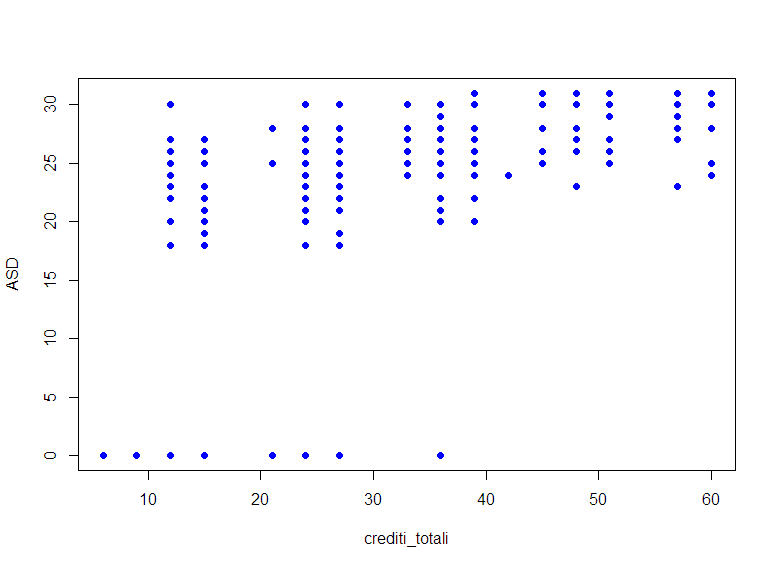
\includegraphics[width=\textwidth]{../img/creditiAsd.png}
      \end{center}
    \end{figure}
  \end{frame}

  \begin{frame}{Scatterplot Crediti totale e ARC}
    \begin{figure}[bt]
      \begin{center}
        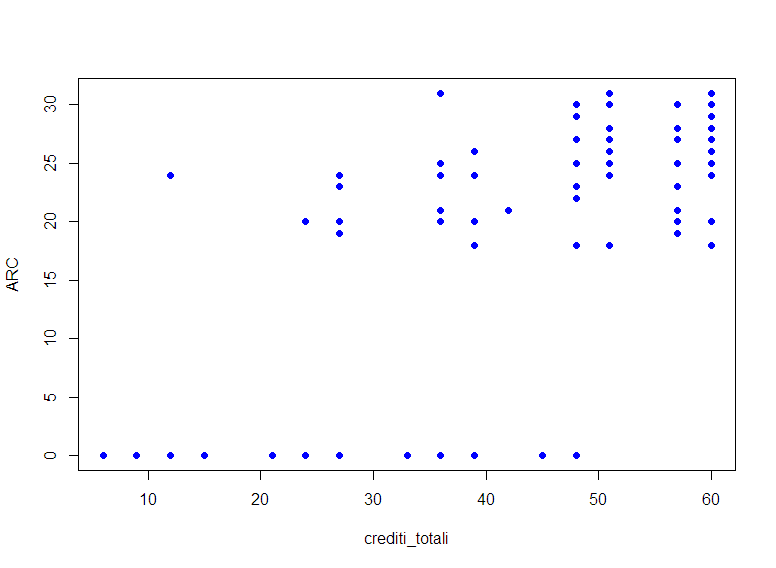
\includegraphics[width=\textwidth]{../img/creditiArc.png}
      \end{center}
    \end{figure}
  \end{frame}

  \begin{frame}{Scatterplot ARC e PRG}
    \begin{figure}[bt]
      \begin{center}
        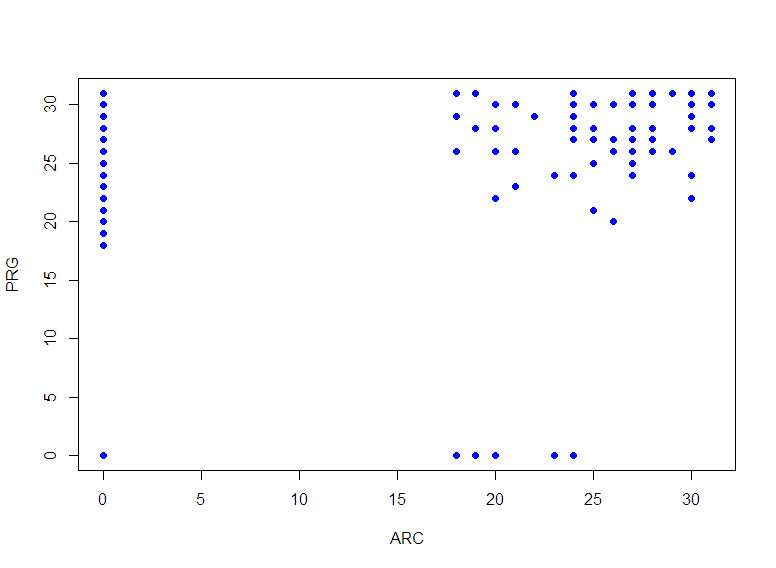
\includegraphics[width=\textwidth]{../img/arcPrg.png}
      \end{center}
    \end{figure}
  \end{frame}

  \begin{frame}{Scatterplot ASD e ANI}
    \begin{figure}[bt]
      \begin{center}
        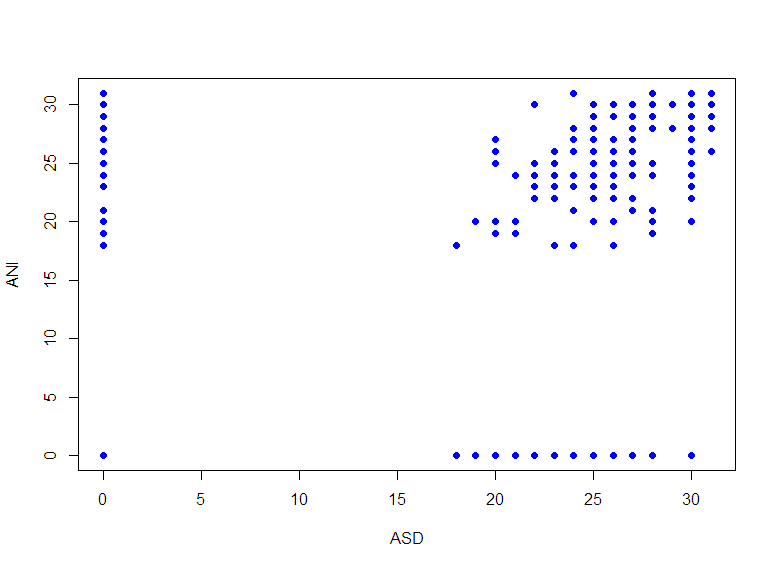
\includegraphics[width=\textwidth]{../img/asdAni.png}
      \end{center}
    \end{figure}
  \end{frame}

  \begin{frame}{Osservazione}
    In uno scatterplot non è
possibile distinguere oggetti con gli stessi valori per gli attributi considerati
e quindi i dati che influenzano maggiormente la correlazione tra Architetture
e Programmazione non vengono essenzialmente mostrati
  \end{frame}
  

  \begin{frame}{Scatterplot ARC e PRG con Jitter}
    \begin{figure}[bt]
      \begin{center}
        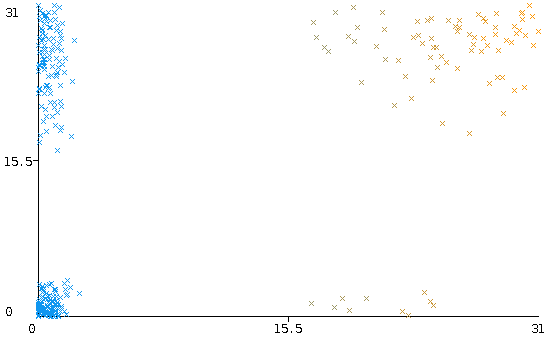
\includegraphics[width=\textwidth]{../img/arcPrgWeka.png}
      \end{center}
    \end{figure}
  \end{frame}

  \begin{frame}{Scatterplot ASD e ANI con Jitter}
    \begin{figure}[bt]
      \begin{center}
        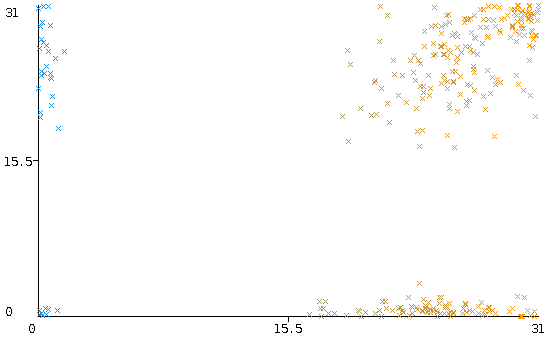
\includegraphics[width=\textwidth]{../img/asdAniWeka.png}
      \end{center}
    \end{figure}
  \end{frame}

  \begin{frame}{Analisi scatterplot con Jitter}
    \begin{enumerate}[-]
      \item Il numero di studenti che non ha sostenuto ne Architteture ne Program\-mazione è notevolmente superiore al numero di studenti che non hanno sostenuto ne algoritmi ne analisi 1. Ciò influenza la correlazione complessiva.
      \item Gli studenti che hanno sostenuto Programmazione ma non hanno sostenuto Architetture sono molti di più rispetto a quelli che hanno sostenuto Analisi 1 ma non hanno sostenuto Algoritmi. Viceversa, gli studenti che hanno sostenuto Architetture ma non Programmazione sono molti meno di quelli che hanno sostenuto Algoritmi ma non Analisi 1. Essendo in quantità paragonabili influenzeranno le correlazione complessive tra le due diverse coppie di attributi circa in egual misura;
    \end{enumerate}
  \end{frame}
  
  \begin{frame}{Analisi scatterplot con Jitter}
    \begin{enumerate}[-]
      \item Confrontando gli studenti che hanno sostenuto sia Architetture che Pro\-grammazione con quelli che hanno sostenuto sia Algoritmi che Analisi 1 si nota una migliore correlazione per la seconda coppia di attributi su tali sottoinsiemi del dataset. Tuttavia, essendo i due sottoinsieme (studenti che hanno sostenuto sia Architetture che Pro\-gramma\-zione e studenti che hanno sostenuto sia Algoritmi che Analisi 1) di dimensioni paragonabili influenzeranno in modo minore la corre\-lazione complessiva rispetto a quanto lo fanno gli studenti discussi nel primo punto.
    \end{enumerate}
  \end{frame}

\begin{frame}{Matrice di correlazione}
  \begin{figure}[bt]
    \begin{center}
      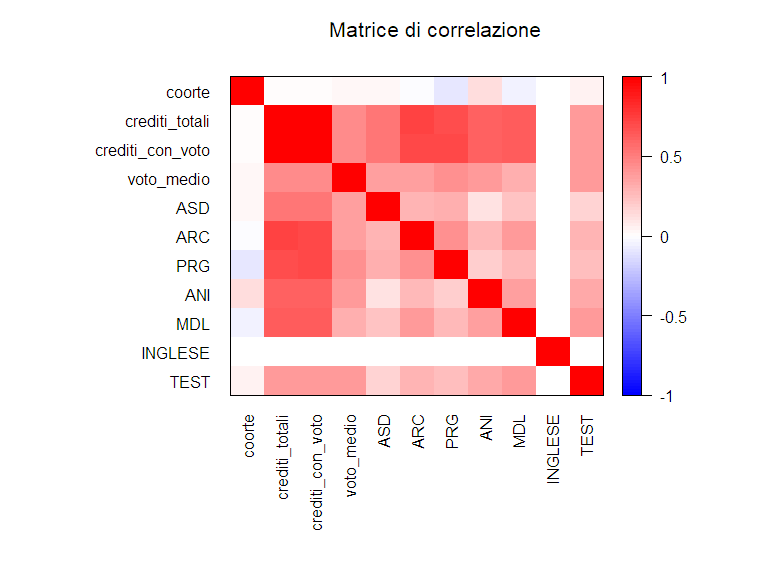
\includegraphics[width=\textwidth]{../img/corMatrix.png}
    \end{center}
  \end{figure}
\end{frame}

\section{Clustering}

\begin{frame}{Clustering}
  \begin{itemize}
    \item crediti totali, architetture, programmazione;
    \item algoritmi e strutture dati, architetture, programmazione, analisi 1 e matematica discreta e logica;
    \item voto medio e test.
  \end{itemize}
\end{frame}

\begin{frame}{Clustering}
  \begin{itemize}
    \item l'analisi effettuata con tecniche di clustering gerarchico è stata effet\-tuata su un sottoinsieme dei dati a disposizione selezionato in base alla coorte dello studente (anno 2010);
    \item nel caso dell'algoritmo di Kmeans viene stabilito preventivamente il numero dei cluster possibili utilizzando valori ritenuti sensati di volta in volta;
    \item l'algoritmo DBSCAN è stato utilizzato per l'analisi relativa ai voti dei diversi esami scegliendo preventivamente i valori di \texttt{MinPts} e \texttt{eps} ritenuti sensati di volta in volta.
  \end{itemize}
\end{frame}

\begin{frame}{Cluster ARC e PRG k = 2}
  \begin{table}[ht]
    \centering
    \begin{tabular}{@{}lllll@{}}
    \toprule
      & Crediti totali & ARC  & PRG  & Istanze\\ \midrule
    0 & 0.65           & 0.32 & 0.85 & 183 ( 58\%)\\
    1 & 0.27           & 0.05 & 0    & 133 ( 42\%)\\ \bottomrule
    \end{tabular}
    \caption{Cluster con ARC e PRG con k = 2 SSE 51.35}
    \label{c2AP}
  \end{table}
\end{frame}

\begin{frame}{Cluster ARC e PRG k = 3}
  \begin{table}[ht]
    \centering
    \begin{tabular}{@{}lllll@{}}
    \toprule
      & Crediti totali & ARC  & PRG  & Istanze\\ \midrule
    0 & 0.88           & 0.82 & 0.89 & 73 ( 23\%)\\
    1 & 0.27           & 0.05 & 0    & 133 ( 42\%)\\
    2 & 0.50           & 0    & 0.81 & 110 ( 35\%)\\ \bottomrule
    \end{tabular}
    \caption{Cluster con ARC e PRG con k = 3 SSE 14.85}
    \label{c3AP}
  \end{table}
\end{frame}

\begin{frame}{Osservazioni}
  \begin{itemize}
    \item Gli studenti appartenenti al cluster 0 sono gli studenti "migliori" a\-vendo sostenuto la quasi totalità degli esami del primo anno alla fine della sessione estiva e riportando delle ottime valutazioni per quanto riguarda gli esami di Architetture e di Programmazione;
    \item La seconda categoria di studenti (cluster 1) sono gli studenti "peg\-giori" che hanno sostenuto pochi esami e nel caso specifico delle materie considerate hanno conseguito valutazioni basse o non hanno sostenuto l'esame;
    \item Infine gli studenti appartenenti all'ultimo cluster sono gli studenti che hanno sostenuto Programmazione con un buon voto ma non hanno fatto l'esame di Architetture.
  \end{itemize}
\end{frame}

\begin{frame}{Osservazioni}
  \begin{itemize}
    \item Non esiste la categoria di studenti che ha sostenuto con profitto l’esame di architetture, ma non ha sostenuto l’esame di programmazione
  \end{itemize}
\end{frame}

\begin{frame}{Dendogramma}
  \begin{figure}[bt]
    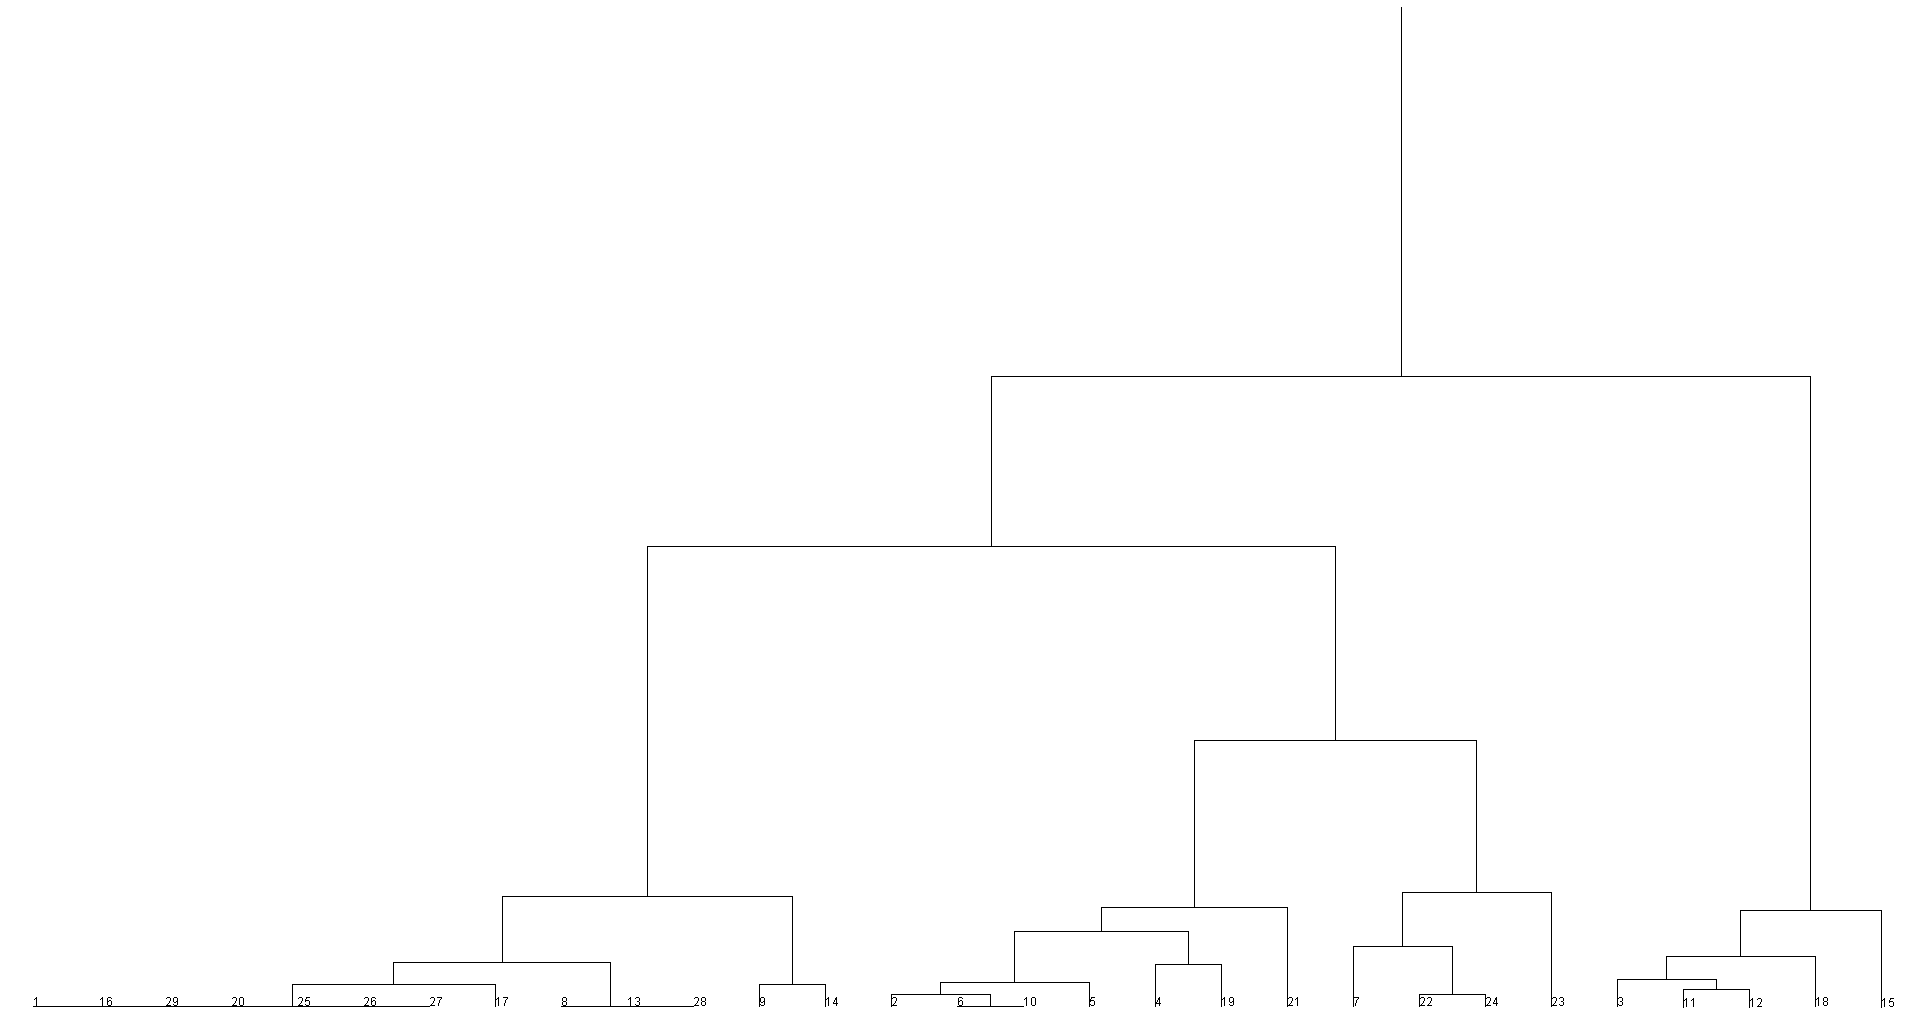
\includegraphics[width=\textwidth]{../img/hierarchical-complete.png}
    \caption{Dendogramma relativo al clustering gerarchico con metodo complete.}
  \end{figure}
\end{frame}

\begin{frame}{Dendogramma}
  \begin{figure}[bt]
    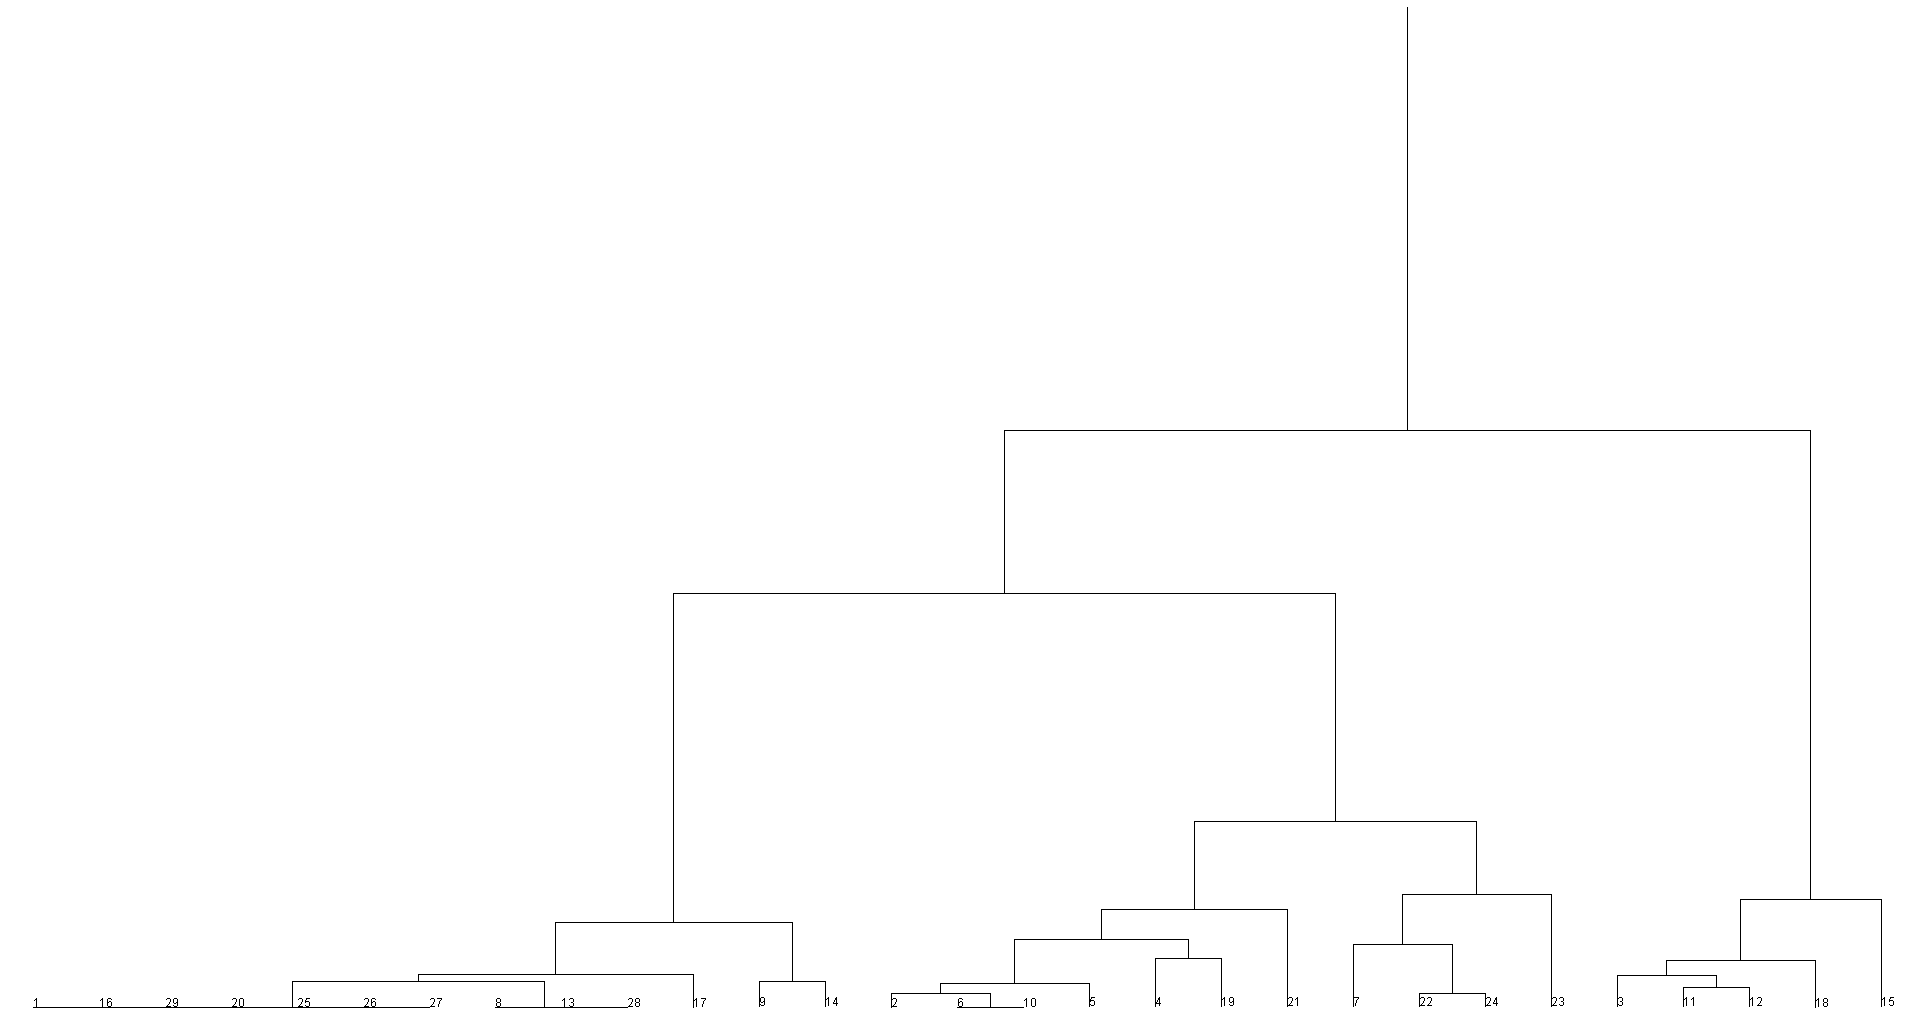
\includegraphics[width=\textwidth]{../img/hierarchical-average.png}
    \caption{Dendogramma relativo al clustering gerarchico con metodo average.}
  \end{figure}
\end{frame}

\begin{frame}{Cluster di tutti i voti}
  \begin{table}[ht]
    \centering
    \begin{tabular}{@{}lllllll@{}}
    \toprule
      & ASD  & ARC  & PRG & ANI  & MDL  & Istanze      \\ \midrule
    0 & 0.73 & 0.05 & 0.81& 0.43 & 0.02 &  100  ( 32\%)\\
    1 & 0.65 & 0.05 & 0   & 0.50 & 0.12 &  133 ( 42\%) \\
    2 & 0.91 & 0.65 & 0.89& 0.88 & 0.60 &  83  ( 26\%) \\ \bottomrule
    \end{tabular}
    \caption{Cluster di tutti i voti con k = 3 SSE 106.19}
    \label{c3V}
  \end{table}
\end{frame}

\begin{frame}{Gruppi di studenti}
  \begin{itemize}
    \item gli studenti che hanno conseguito una buona votazione negli esami di Algoritmi e Strutture Dati e Programmazione,
    una votazione dis\-creta all'esame di Analisi I e che non hanno sostenuto Matematica discreta e Logica e Architetture degli elaboratori;
    \item gli studenti con le stesse caratteristiche del cluster precedente, ma che hanno sostenuto Programmazione
    \item gli studenti che hanno sostenuto tutti gli esami e con un buona vota\-zione.
  \end{itemize}
\end{frame}

\begin{frame}{Scatter plot dei cluster}
  \begin{figure}[bt]
    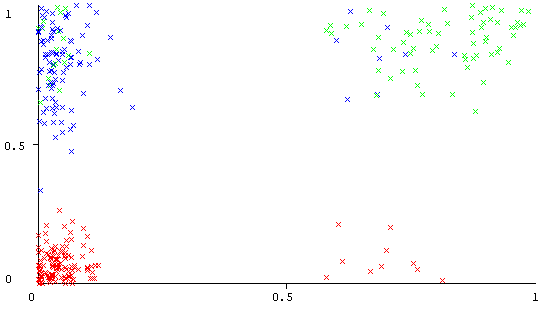
\includegraphics[width=\textwidth]{../img/ARC-PRG-Cluster.png}
    \caption{Scatter plot relativo ai cluster dei voti di Architetture degli Elaboratori e Programmazione}
  \end{figure}
\end{frame}

\begin{frame}{Cluster DBSCAN}
  \begin{table}[H]
    \centering
    \begin{tabular}{@{}ll@{}}
    \toprule
                            & Istanze  \\\midrule
    \multicolumn{1}{l}{0} & 40 (14\%)  \\
    \multicolumn{1}{l}{1} & 46 (17\%)  \\
    \multicolumn{1}{l}{2} & 41 (15\%)  \\
    \multicolumn{1}{l}{3} & 13 (5\%)   \\
    \multicolumn{1}{l}{4} & 45 (16\%)  \\
    \multicolumn{1}{l}{5} & 33 (12\%)  \\
    \multicolumn{1}{l}{6} & 6  (2\%)   \\
    \multicolumn{1}{l}{7} & 18 (6\%)   \\
    \multicolumn{1}{l}{8} & 22 (8\%)   \\
    \multicolumn{1}{l}{9} & 14 (5\%)   \\\bottomrule
    \end{tabular}
    \caption{Cluster ottenuti con DBSCAN eseguito con \texttt{MinPts=6} e \texttt{eps=0.5}.}
    \end{table}
\end{frame}


\begin{frame}{Osservazioni}
  \begin{itemize}
    \item 38 record dei 316 totali sono stati marcati come rumore dall’algoritmo
    \item Cluster di piccole dimensioni
    \item \texttt{MinPts} troppo basso
  \end{itemize}
\end{frame}

\begin{frame}{Cluster DBSCAN}
  \begin{table}[H]
    \centering
    \begin{tabular}{@{}ll@{}}
    \toprule
                            & Istanze    \\ \midrule
    \multicolumn{1}{l}{0}   & 40 (15\%)  \\ 
    \multicolumn{1}{l}{1}   & 46 (17\%)  \\ 
    \multicolumn{1}{l}{2}   & 41 (15\%)  \\ 
    \multicolumn{1}{l}{3}   & 13 (5\%)   \\ 
    \multicolumn{1}{l}{4}   & 45 (17\%)  \\ 
    \multicolumn{1}{l}{5}   & 33 (12\%)  \\ 
    \multicolumn{1}{l}{6}   & 18 (7\%)   \\ 
    \multicolumn{1}{l}{7}   & 22 (8\%)   \\ 
    \multicolumn{1}{l}{8}   & 14 (5\%)   \\ \bottomrule
    \end{tabular}
    \caption{Cluster ottenuti con DBSCAN eseguito con \texttt{MinPts=10} e \texttt{eps=0.4}.}
    \end{table}
\end{frame}

\begin{frame}{Osservazioni}
  \begin{itemize}
    \item 44 record dei 316 totali sono stati marcati come rumore dall’algoritmo
    \item Il numero dei cluster diminuisce e passa a 8
    \item I cluster di piccole dimensioni diventano solo due
  \end{itemize}
\end{frame}

\begin{frame}{Cluster DBSCAN}
  \begin{table}[H]
    \centering
    \begin{tabular}{@{}ll@{}}
    \toprule
                            & Istanze  \\ \midrule
    \multicolumn{1}{l}{0} & 40 (18\%) \\
    \multicolumn{1}{l}{1} & 46 (20\%) \\
    \multicolumn{1}{l}{2} & 41 (18\%) \\
    \multicolumn{1}{l}{3} & 45 (20\%) \\
    \multicolumn{1}{l}{4} & 33 (15\%) \\
    \multicolumn{1}{l}{5} & 22 (10\%) \\ \bottomrule
    \end{tabular}
    \caption{Cluster ottenuti con DBSCAN eseguito con \texttt{MinPts=20} e \texttt{eps=0.4}.}
    \end{table}
\end{frame}

\begin{frame}{Osservazioni}
  \begin{itemize}
    \item 89 record dei 316 totali sono stati marcati come rumore dall’algoritmo
    \item Il numero dei cluster è pari a 6
    \item La distribuzione dei record nei cluster risulta decisamente più uniforme
    \item I cluster di piccole dimensioni non sono presenti
  \end{itemize}
\end{frame}

\begin{frame}{Cluster Voto medio e Test}
  \begin{table}[ht]
    \centering
    \begin{tabular}{@{}llll@{}}
    \toprule
      & voto medio & Test  & Istanze\\ \midrule
    0 & 0.36       & 0.41  & 85  ( 27\%)\\
    1 & 0.75       & 0.66  & 146 ( 42\%)\\
    2 & 0.45       & 0.67  & 85  ( 27\%)\\ \bottomrule
    \end{tabular}
    \caption{Cluster con Voto\_medio e Test con k = 3 SSE 9.6}
    \label{c3MT}
  \end{table}
\end{frame}

\begin{frame}{Osservazioni}
  \begin{itemize}
    \item Si determinano tre cluster ben distinti
    \item I primi due cluster identificano gli studenti "migliori" e quelli "peggiori"
    \item Nel terzo cluster gli studenti hanno conseguito un punteggio al test d’ingresso decisamente positivo, ma non hanno mantenuto una media dei voti altrettanto buona
  \end{itemize}
\end{frame}

\section{Valutazione del clustering e model selection}

\begin{frame}{Valutazione del clustering e model selection} 
    \begin{itemize}
      \item Selezione del numero "ottimale" di cluster per il K-means
      \item Valutazione del K-means
      \item Valutazione DBSCAN
    \end{itemize} 
\end{frame}

\begin{frame}{Selezione numero di cluster nel K-means} 
    Viene effettuata tramite la seguente procedura
    \begin{itemize}
      \item Determinazione SSE in funzione di $k$
      \item Selezione del valore ottimale di $k_{opt}$ 
    \end{itemize} 
    successivamente è possibile valutare e confrontare i risultati ottenuti dall'algoritmo
    con i diversi valori di $k$.
\end{frame}

\begin{frame}{Example}
    \begin{figure}[bt]
      \begin{center}
      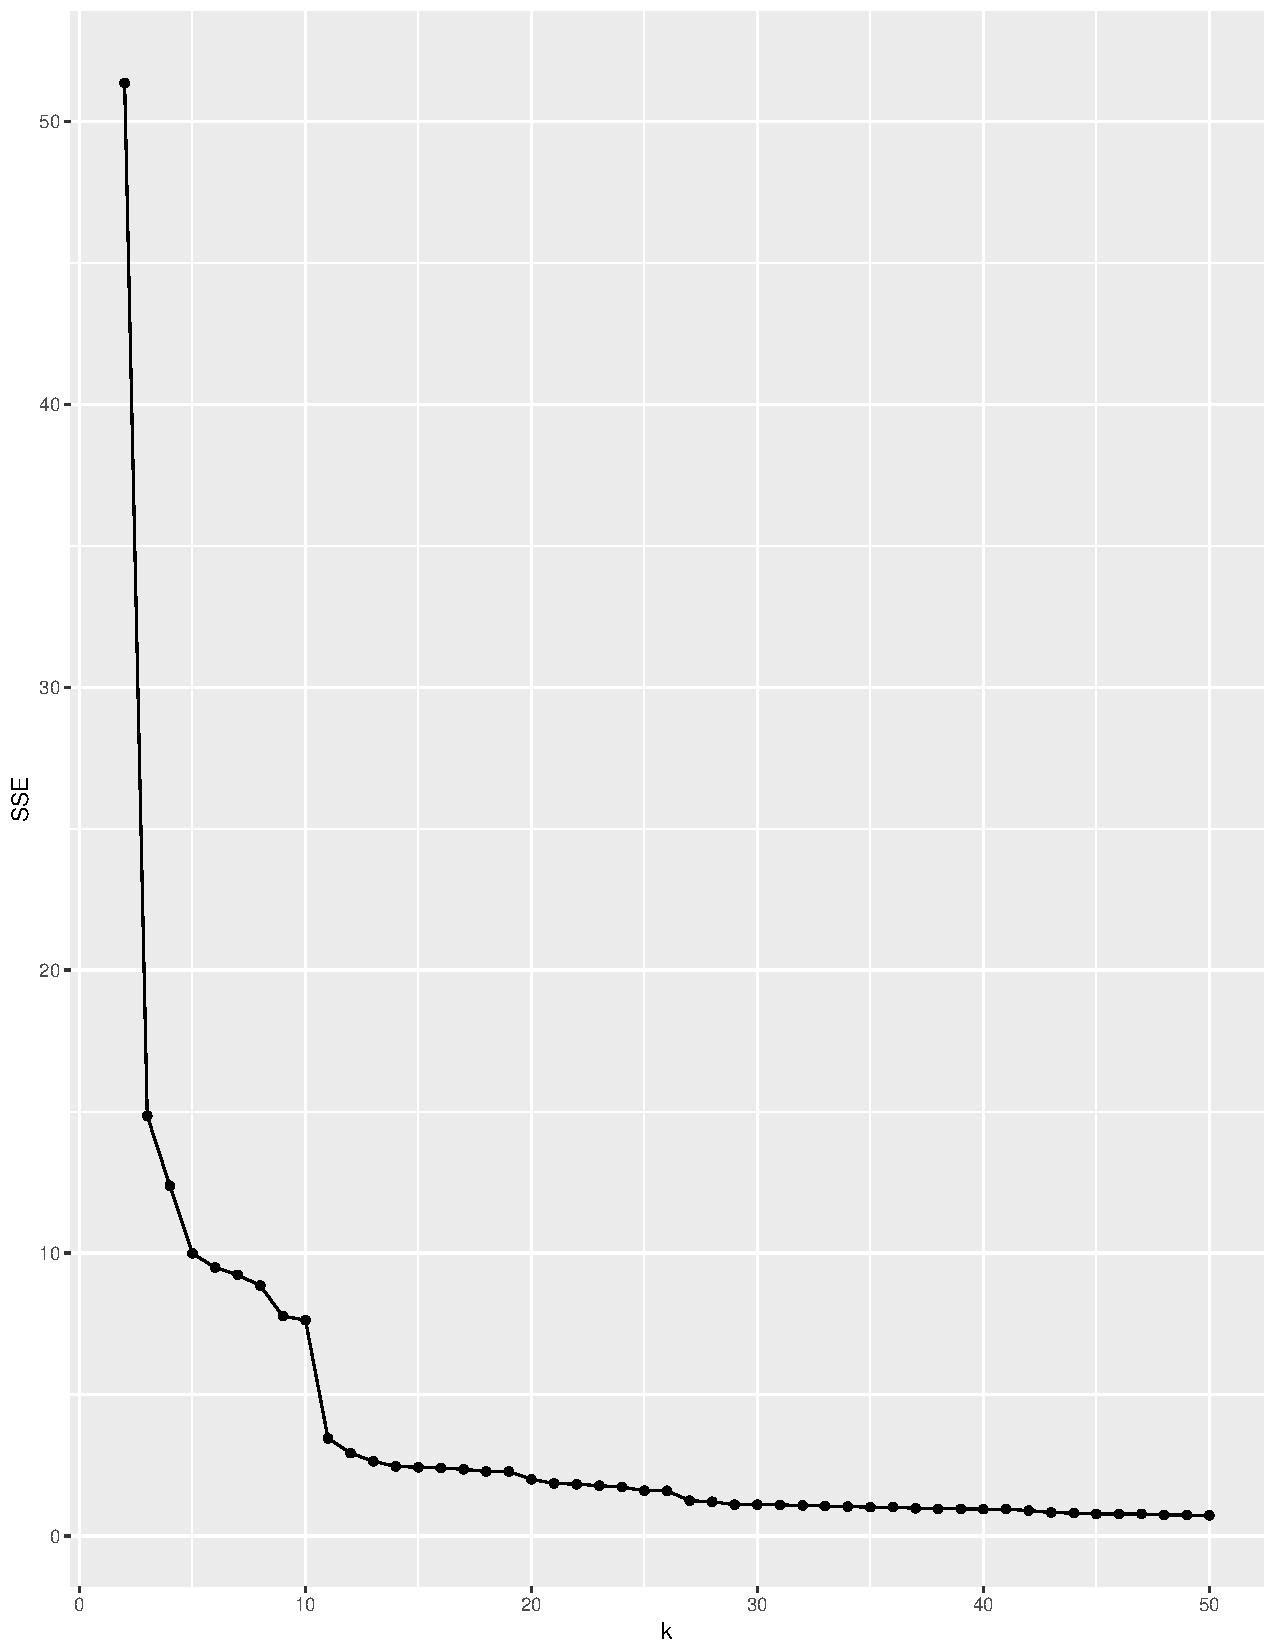
\includegraphics[width = 0.45\textwidth]{../img/k-sse-crediti-totali-arc-prg.pdf}
      \caption{Dependency update}
      \end{center}
    \end{figure}
\end{frame}

\begin{frame}{Example}
  \begin{figure}[bt]
    \begin{center}
    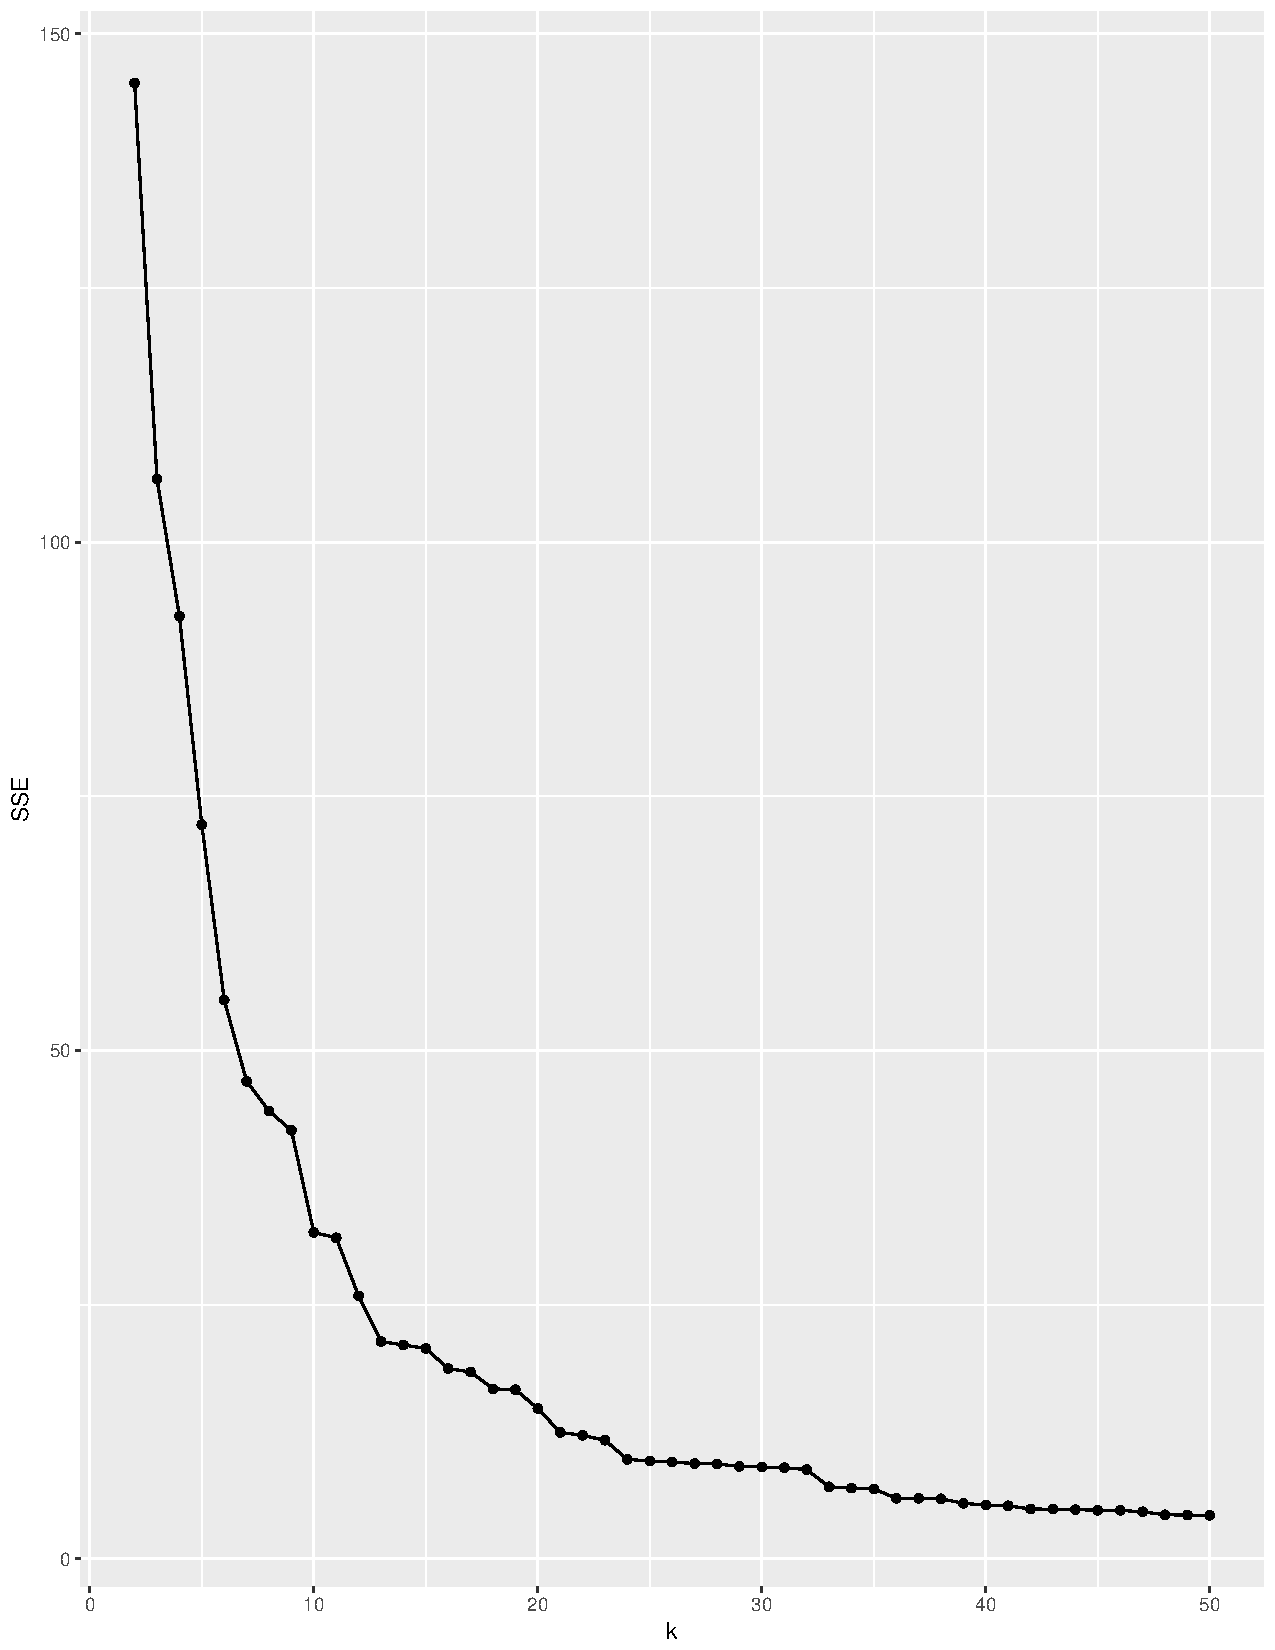
\includegraphics[width = 0.45\textwidth]{../img/k-sse-asd-arc-prg-an1-mdl.pdf}
    \caption{Dependency update}
    \end{center}
  \end{figure}
\end{frame}

\begin{frame}{Example}
    \begin{figure}[bt]
      \begin{center}
      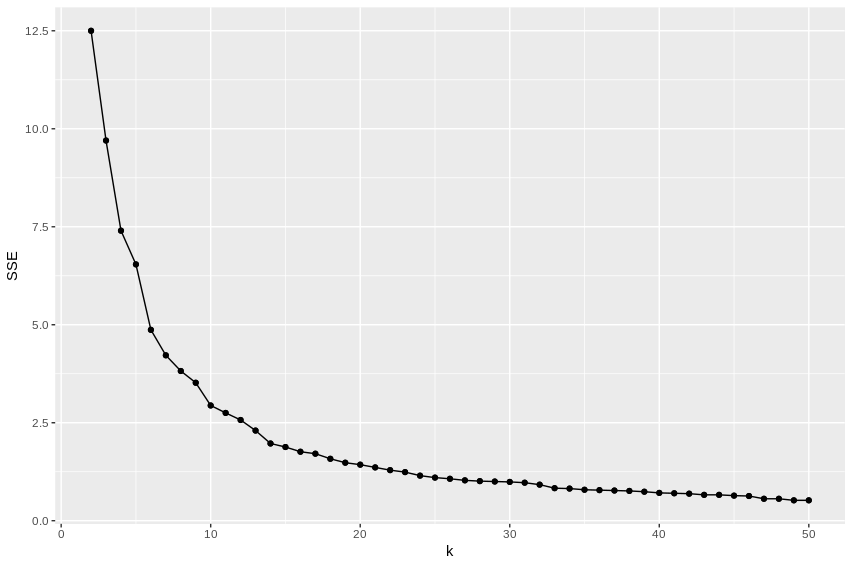
\includegraphics[width = 0.45\textwidth]{../img/k-sse-voto_medio-test.png}
      \caption{Dependency update}
      \end{center}
    \end{figure}
\end{frame}

\begin{frame}{Selezione \texttt{Eps} fissato \texttt{MinPts} in DBSCAN} 
    Viene effettuata tramite la seguente procedura
    \begin{itemize}
      \item Ordino i punti rispetto alla loro distanza dal loro $k$-esimo punto più vicino
      item pongo \texttt{MinPts}=$k$
      \item Determino un grafico con indici punti ordinati e distanze dal $k$-esimo più vicino 
      \item Selezione come valore di \texttt{Eps} quello per cui c'è un picco.
    \end{itemize} 
\end{frame}

\begin{frame}{Valutazione} 
    La valutazione dei clustering ottenuti con K-means e DBSCAN è stata fatta con la seguente procedura
    \begin{itemize}
      \item Calcolo matrice distanze tra i punti
      \item Calcolo matrice di incidenza dei cluster
      \item "Serializzazione" e calcolo della correlazione
    \end{itemize} 
    successivamente è possibile valutare e confrontare i risultati ottenuti dai clustering ottenuti
    con il K-means con i diversi valori di $k$ e con il DBSCAN.
\end{frame}

\begin{frame}[fragile]{SQL}
\begin{lstlisting}[style = R]
# Matrice di incidenza
matriceIncidenza <- function(data){
  nr = nrow(data)
  nc = ncol(data)
  C = matrix(nrow = nr, ncol = nr)
  for(i in 1:nr){
    for(j in 1:nr){
      if(data[i,nc] == data[j,nc])
        C[i,j] = 1
      else
        C[i,j] = 0
    }
  }
return(C)
\end{lstlisting}
\end{frame}

\begin{frame}[fragile]{SQL}
\begin{lstlisting}[style = R]
# matrice distanza
matriceDistanza <- function(data){
  return(as.matrix(dist(data[,1:(ncol(data)-1)],method = 'euclidean',diag = TRUE,upper = TRUE)))
}

calcoloCorrelazione <- function(data){
  MI <- matriceIncidenza(data)
  D <- matriceDistanza(data)
  mi = as.vector(t(MI))
  d = as.vector(t(D))
  
  return(cor(mi,d,method="pearson"))
}

calcoloCorrelazione(crediti_totali_prg_arc_clustered)
\end{lstlisting}
\end{frame}

\begin{frame}{Valori Correlazione K-means}
  % tabella 9 relazione
  \begin{table}[H]
      \centering
      \resizebox{\textwidth}{!}{
      \begin{tabular}{@{}llllllllllll@{}}
                         & coorte   & crediti totali & crediti con voto  & voto medio  & ASD      & ARC      & PRG     & ANI     & MDL      & ING & TEST    \\ \midrule
      coorte             & 1        & 0.013343        & 0.01821             & 0.03655      & 0.03581  & -0.01609 & -0.0822 & 0.13386 & -0.04033 & NA      & 0.04126 \\ 
      crediti\_totali    & 0.01334  & 1               & 0.99522             & 0.44571      & 0.52984  & 0.72508  & 0.69882 & 0.61015 & 0.62789  & NA      & 0.38433 \\
      crediti\_con\_voto & 0.01821  & 0.99522         & 1                   & 0.44838      & 0.52957  & 0.71955  & 0.70879 & 0.61593 & 0.62654  & NA      & 0.39025 \\
      voto\_medio        & 0.03655  & 0.44571         & 0.44838             & 1            & 0.36900  & 0.36427  & 0.43085 & 0.39777 & 0.31828  & NA      & 0.39428 \\
      ASD                & 0.03581  & 0.52984         & 0.52957             & 0.36900      & 1        & 0.29321  & 0.31192 & 0.10116 & 0.23775  & NA      & 0.16149 \\
      ARC                & -0.0160  & 0.72508         & 0.71955             & 0.36427      & 0.29321  & 1        & 0.43166 & 0.27541 & 0.39622  & NA      & 0.29979 \\
      PRG                & -0.0822  & 0.69882         & 0.70879             & 0.43085      & 0.31192  & 0.43166  & 1       & 0.19585 & 0.27295  & NA      & 0.24356 \\
      ANI                & 0.13386  & 0.61015         & 0.61593             & 0.39777      & 0.10116  & 0.27541  & 0.19585 & 1       & 0.36333  & NA      & 0.32378 \\
      MDL                & -0.0403  & 0.62789         & 0.62654             & 0.31828      & 0.23775  & 0.39622  & 0.27295 & 0.36333 & 1        & NA      & 0.38777 \\
      ING                & NA       & NA              & NA                  & NA           & NA       & NA       & NA      & NA      & NA       & 1       & NA      \\ 
      TEST               & 0.04126  & 0.384332        & 0.39025             & 0.39428      & 0.16149  & 0.29979  & 0.2435  & 0.32378 & 0.38777  & NA      & 1       \\\bottomrule                 
      \end{tabular}
      }
  \end{table}
\end{frame}

\begin{frame}{Valutazione k-Means} 
    \begin{itemize}
      \item Procedura model selection non efficace
      \item Valori scelti inizialmente sono migliori
    \end{itemize} 
\end{frame}

\begin{frame}{Valutazione DBSCAN} 
  \begin{itemize}
    \item E' possibile calcolare lo stesso valore di correlazione anche per il DBSCAN
    \item Necessaria preventiva rimozione di rumore
  \end{itemize} 
\end{frame}

\begin{frame}{Rimozione rumore con Weka}
  \begin{figure}[bt]
    \begin{center}
    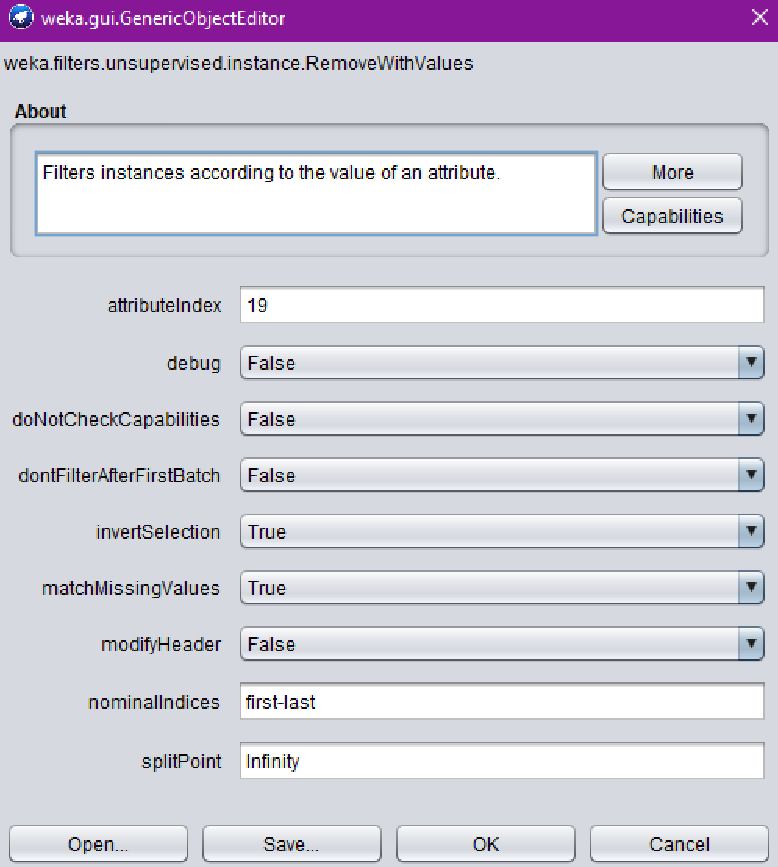
\includegraphics[width = 0.45\textwidth]{../img/filter-for-remove-noise.pdf}
    \caption{Dependency update}
    \end{center}
  \end{figure}
\end{frame}

\begin{frame}{Correlazione e rumore DBSCAN}
  % tabella 10
  \begin{table}[H]
      \centering
      \resizebox{\textwidth}{!}{
      \begin{tabular}{@{}llllllllllll@{}}
                         & coorte   & crediti totali & crediti con voto  & voto medio  & ASD      & ARC      & PRG     & ANI     & MDL      & ING & TEST    \\ \midrule
      coorte             & 1        & 0.013343        & 0.01821             & 0.03655      & 0.03581  & -0.01609 & -0.0822 & 0.13386 & -0.04033 & NA      & 0.04126 \\ 
      crediti\_totali    & 0.01334  & 1               & 0.99522             & 0.44571      & 0.52984  & 0.72508  & 0.69882 & 0.61015 & 0.62789  & NA      & 0.38433 \\
      crediti\_con\_voto & 0.01821  & 0.99522         & 1                   & 0.44838      & 0.52957  & 0.71955  & 0.70879 & 0.61593 & 0.62654  & NA      & 0.39025 \\
      voto\_medio        & 0.03655  & 0.44571         & 0.44838             & 1            & 0.36900  & 0.36427  & 0.43085 & 0.39777 & 0.31828  & NA      & 0.39428 \\
      ASD                & 0.03581  & 0.52984         & 0.52957             & 0.36900      & 1        & 0.29321  & 0.31192 & 0.10116 & 0.23775  & NA      & 0.16149 \\
      ARC                & -0.0160  & 0.72508         & 0.71955             & 0.36427      & 0.29321  & 1        & 0.43166 & 0.27541 & 0.39622  & NA      & 0.29979 \\
      PRG                & -0.0822  & 0.69882         & 0.70879             & 0.43085      & 0.31192  & 0.43166  & 1       & 0.19585 & 0.27295  & NA      & 0.24356 \\
      ANI                & 0.13386  & 0.61015         & 0.61593             & 0.39777      & 0.10116  & 0.27541  & 0.19585 & 1       & 0.36333  & NA      & 0.32378 \\
      MDL                & -0.0403  & 0.62789         & 0.62654             & 0.31828      & 0.23775  & 0.39622  & 0.27295 & 0.36333 & 1        & NA      & 0.38777 \\
      ING                & NA       & NA              & NA                  & NA           & NA       & NA       & NA      & NA      & NA       & 1       & NA      \\ 
      TEST               & 0.04126  & 0.384332        & 0.39025             & 0.39428      & 0.16149  & 0.29979  & 0.2435  & 0.32378 & 0.38777  & NA      & 1       \\\bottomrule                 
      \end{tabular}
      }
  \end{table}
\end{frame}

\begin{frame}[fragile]{Model selection DBSCAN}
  % codice 6 relazione
  \begin{lstlisting}[style=sql]
      Hello world  
  \end{lstlisting}
\end{frame}

\begin{frame}{Rimozione rumore con Weka}
  \begin{figure}[bt]
    \begin{center}
    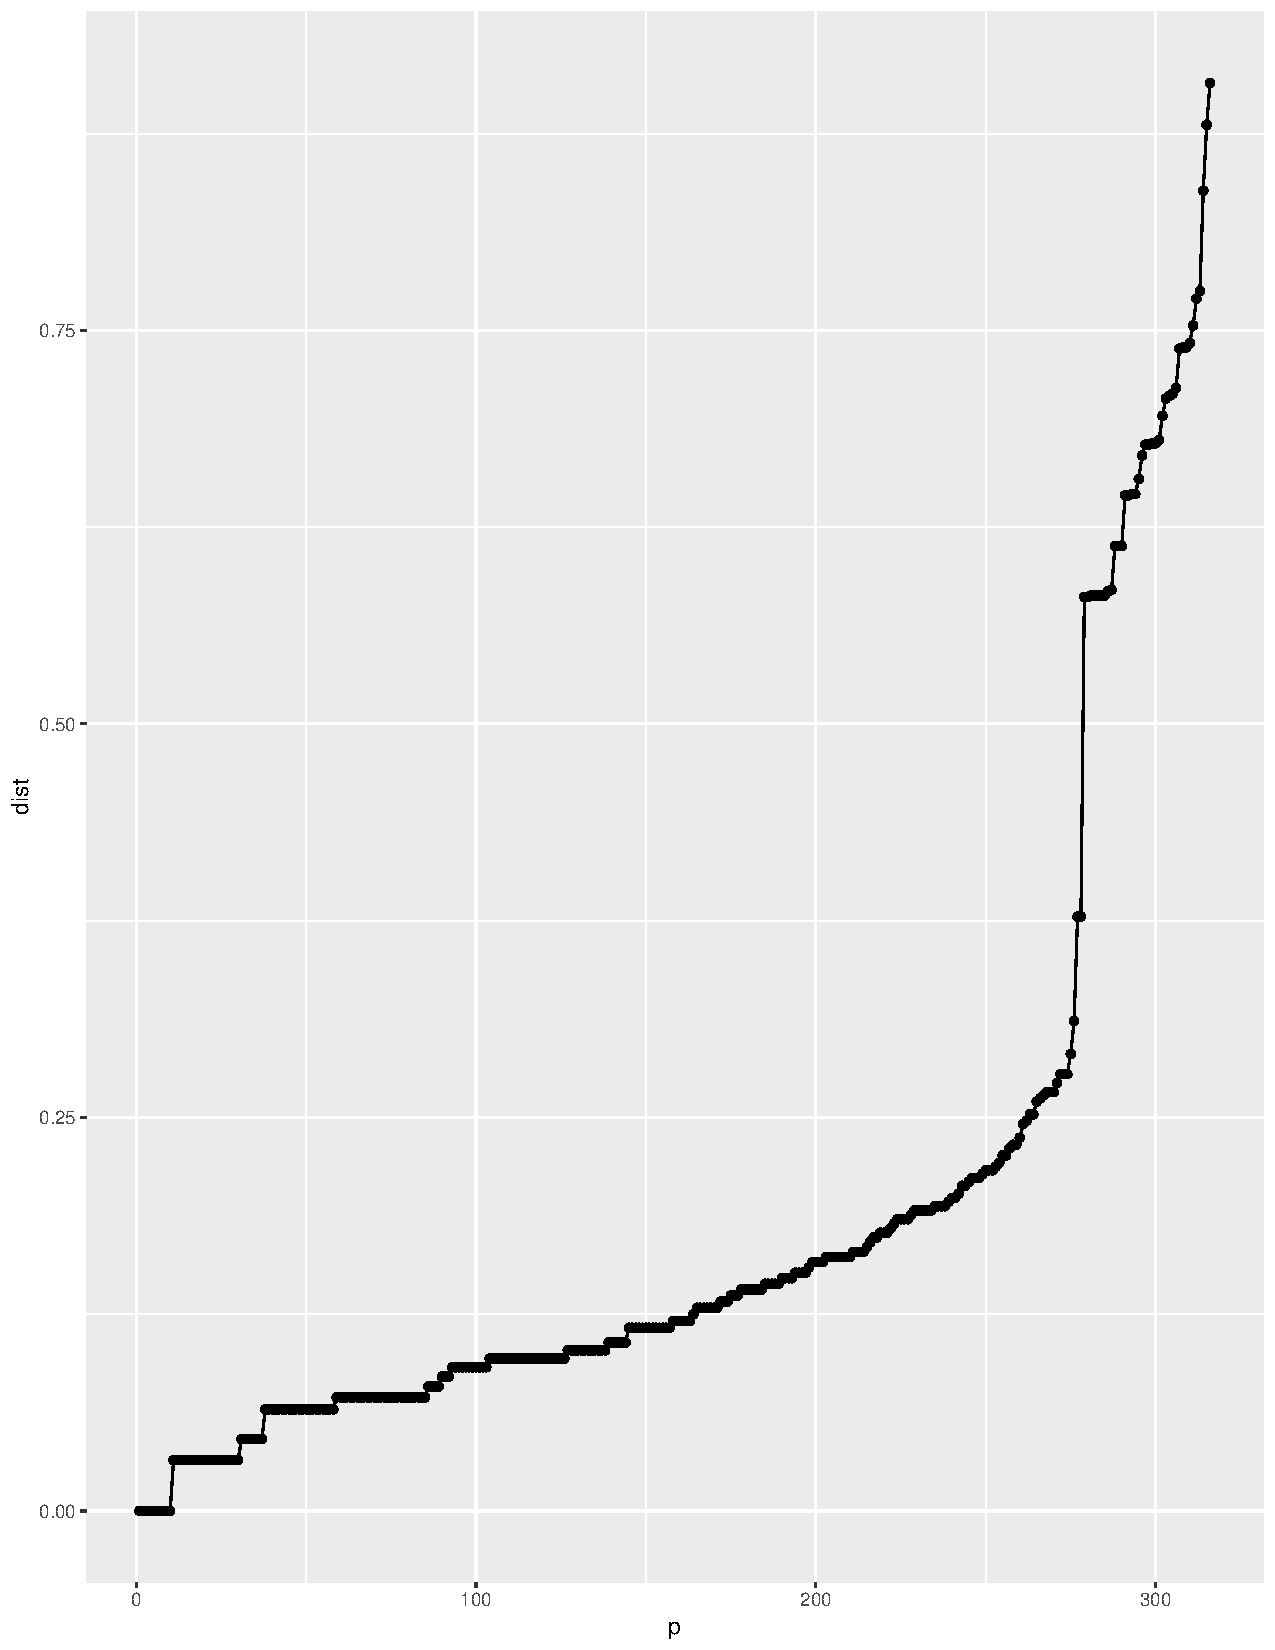
\includegraphics[width = 0.45\textwidth]{../img/eps-minpts6.pdf}
    \caption{Dependency update}
    \end{center}
  \end{figure}
\end{frame}

\begin{frame}{Rimozione rumore con Weka}
  \begin{figure}[bt]
    \begin{center}
    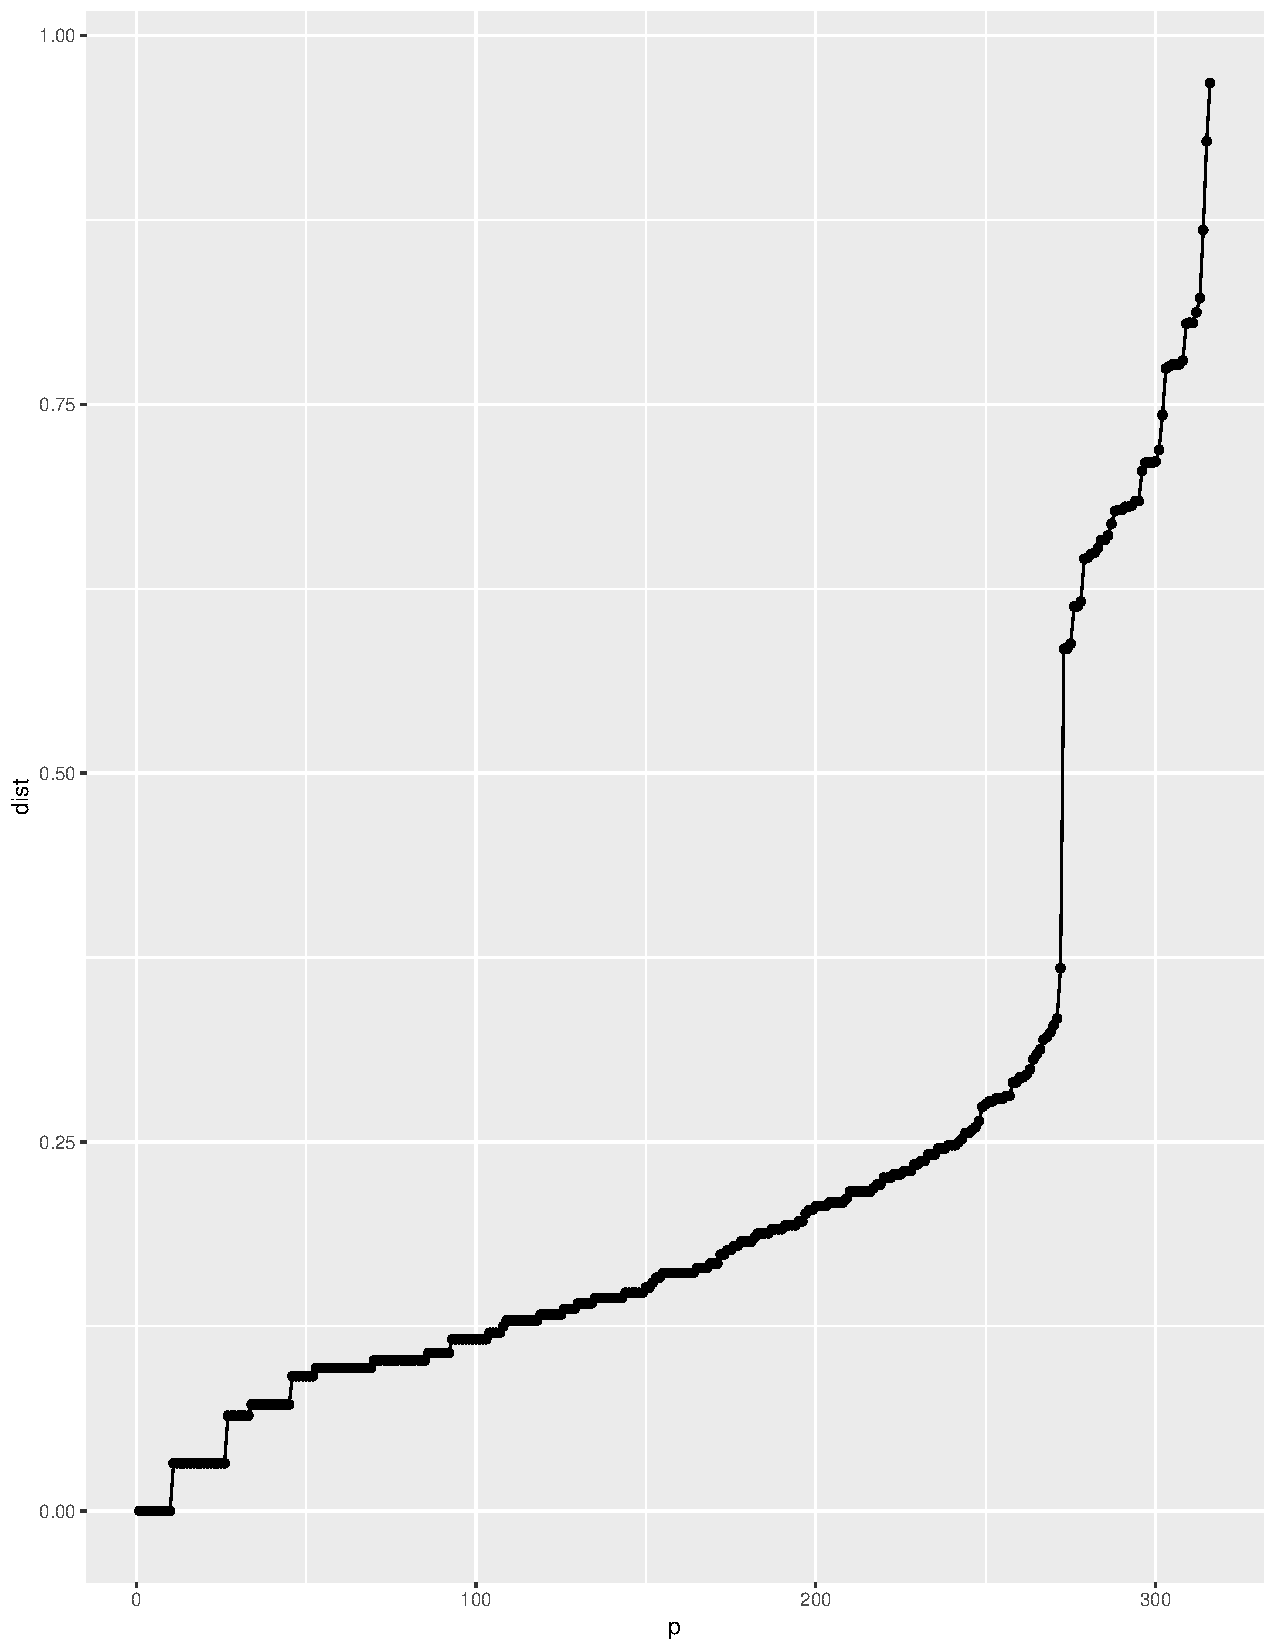
\includegraphics[width = 0.45\textwidth]{../img/eps-minpts10.pdf}
    \caption{Dependency update}
    \end{center}
  \end{figure}
\end{frame}

\begin{frame}{Rimozione rumore con Weka}
  \begin{figure}[bt]
    \begin{center}
    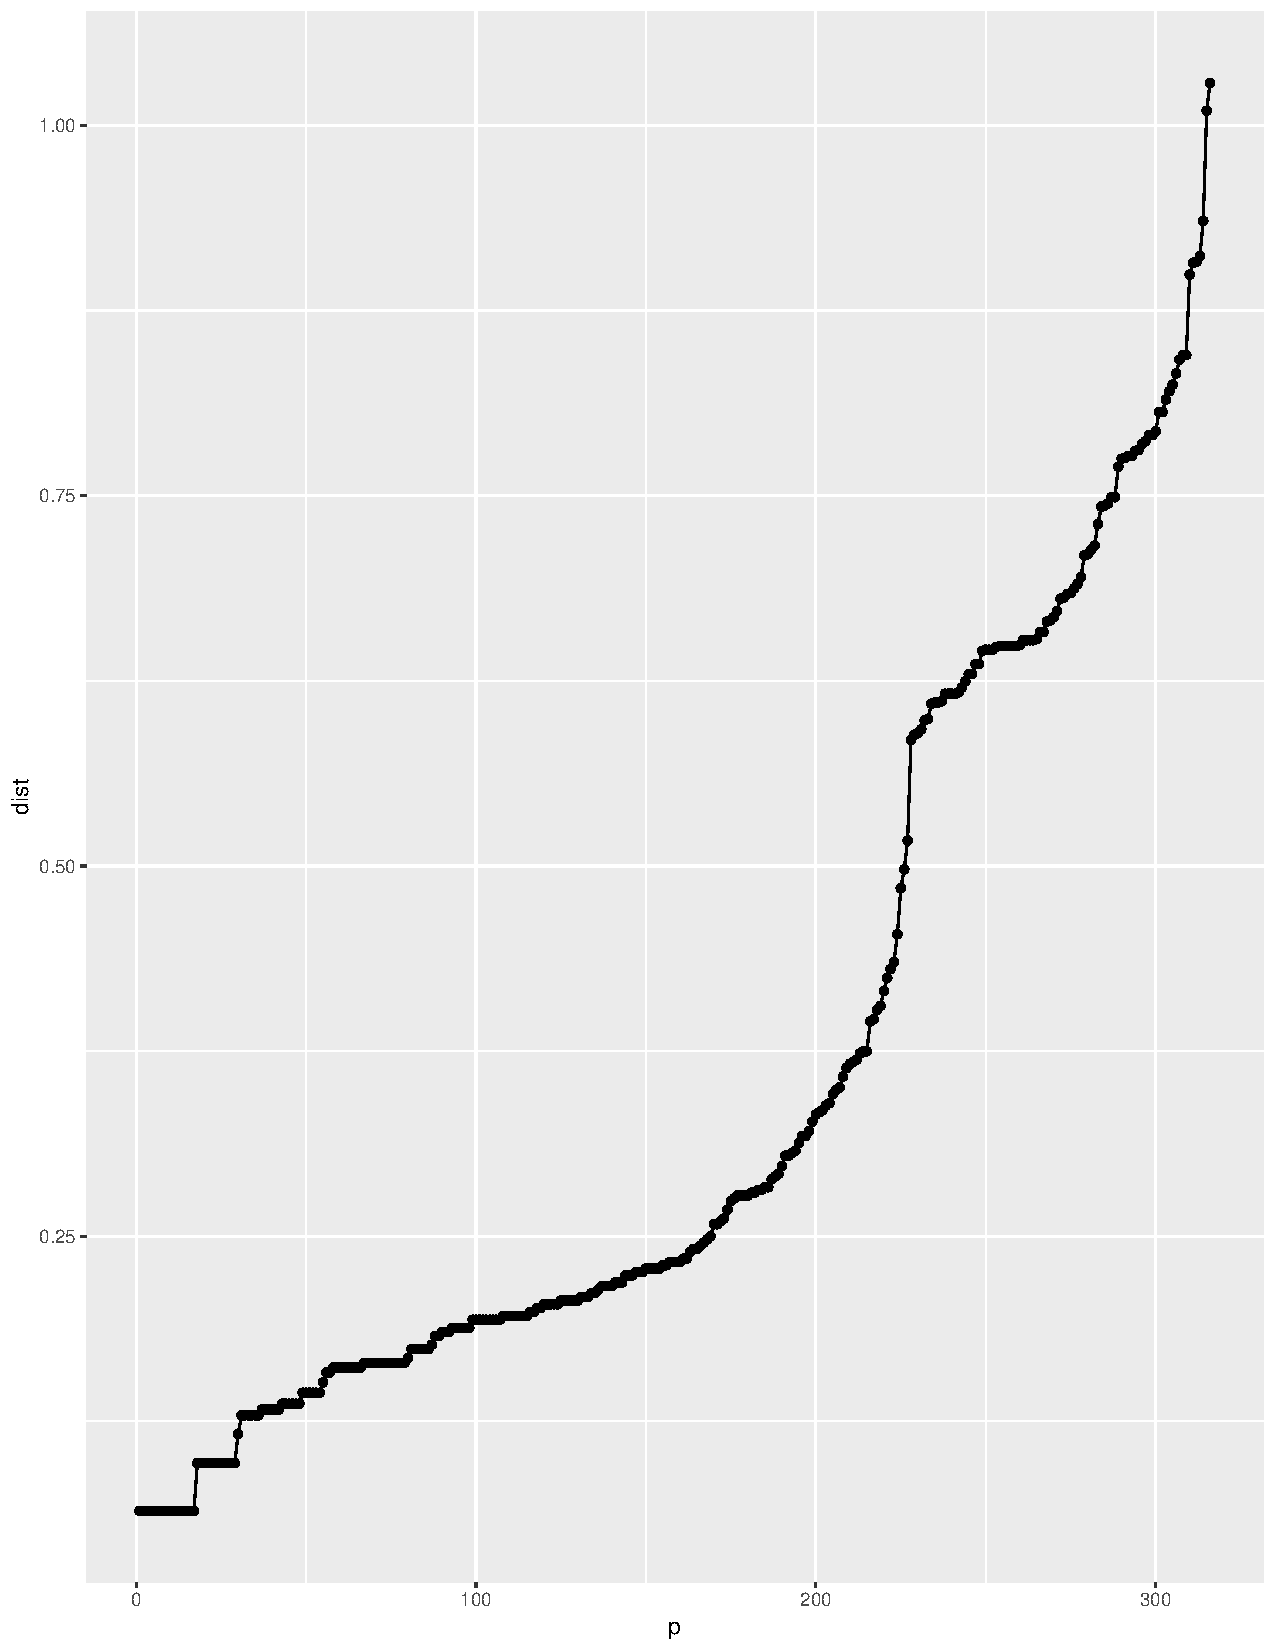
\includegraphics[width = 0.45\textwidth]{../img/eps-minpts20.pdf}
    \caption{Dependency update}
    \end{center}
  \end{figure}
\end{frame}

\begin{frame}{Correlazione e rumore DBSCAN}
  % tabella 11
  \begin{table}[H]
      \centering
      \resizebox{\textwidth}{!}{
      \begin{tabular}{@{}llllllllllll@{}}
                         & coorte   & crediti totali & crediti con voto  & voto medio  & ASD      & ARC      & PRG     & ANI     & MDL      & ING & TEST    \\ \midrule
      coorte             & 1        & 0.013343        & 0.01821             & 0.03655      & 0.03581  & -0.01609 & -0.0822 & 0.13386 & -0.04033 & NA      & 0.04126 \\ 
      crediti\_totali    & 0.01334  & 1               & 0.99522             & 0.44571      & 0.52984  & 0.72508  & 0.69882 & 0.61015 & 0.62789  & NA      & 0.38433 \\
      crediti\_con\_voto & 0.01821  & 0.99522         & 1                   & 0.44838      & 0.52957  & 0.71955  & 0.70879 & 0.61593 & 0.62654  & NA      & 0.39025 \\
      voto\_medio        & 0.03655  & 0.44571         & 0.44838             & 1            & 0.36900  & 0.36427  & 0.43085 & 0.39777 & 0.31828  & NA      & 0.39428 \\
      ASD                & 0.03581  & 0.52984         & 0.52957             & 0.36900      & 1        & 0.29321  & 0.31192 & 0.10116 & 0.23775  & NA      & 0.16149 \\
      ARC                & -0.0160  & 0.72508         & 0.71955             & 0.36427      & 0.29321  & 1        & 0.43166 & 0.27541 & 0.39622  & NA      & 0.29979 \\
      PRG                & -0.0822  & 0.69882         & 0.70879             & 0.43085      & 0.31192  & 0.43166  & 1       & 0.19585 & 0.27295  & NA      & 0.24356 \\
      ANI                & 0.13386  & 0.61015         & 0.61593             & 0.39777      & 0.10116  & 0.27541  & 0.19585 & 1       & 0.36333  & NA      & 0.32378 \\
      MDL                & -0.0403  & 0.62789         & 0.62654             & 0.31828      & 0.23775  & 0.39622  & 0.27295 & 0.36333 & 1        & NA      & 0.38777 \\
      ING                & NA       & NA              & NA                  & NA           & NA       & NA       & NA      & NA      & NA       & 1       & NA      \\ 
      TEST               & 0.04126  & 0.384332        & 0.39025             & 0.39428      & 0.16149  & 0.29979  & 0.2435  & 0.32378 & 0.38777  & NA      & 1       \\\bottomrule                 
      \end{tabular}
      }
  \end{table}
\end{frame}

\section{Conclusioni}

\begin{frame}{Conclusioni} 
    \begin{itemize}
      \item Architetture degli elaboratori esame più difficile
      \item La media alla fine del primo anno non sempre conferma i risultati ottenuti al test di ingresso
      \item Non tutti gli esami sono generalmente sostenuti al primo anno
    \end{itemize} 
\end{frame}

\begin{frame}
  \begin{center}
  \Huge Grazie per l'attenzione
  \end{center}
\end{frame}
\end{document}